
%(BEGIN_QUESTION)
% Copyright 2006, Tony R. Kuphaldt, released under the Creative Commons Attribution License (v 1.0)
% This means you may do almost anything with this work of mine, so long as you give me proper credit

An ohmmeter registers a resistance of 5.8 k$\Omega$ when connected between two metal plates immersed in a sample of water.  The metal plates each measure 3 centimeters by 3 centimeters, and are separated by a distance of 10 centimeters:

$$\includegraphics[width=15.5cm]{i00923x01.eps}$$

Calculate the specific conductivity of this water, expressed in units of microsiemens per centimeter ($\mu$S/cm):

\vskip 10pt

Specific conductivity = \underbar{\hskip 50pt} $\mu$S/cm

\underbar{file i00923}
%(END_QUESTION)





%(BEGIN_ANSWER)

Specific conductivity = \underbar{\bf 191.57} $\mu$S/cm

%(END_ANSWER)





%(BEGIN_NOTES)

%INDEX% Measurement, analytical: conductivity

%(END_NOTES)


